% Q17: 按固定候选 PDF 第1页（印刷页282）空间图重绘；不表示长度比例。
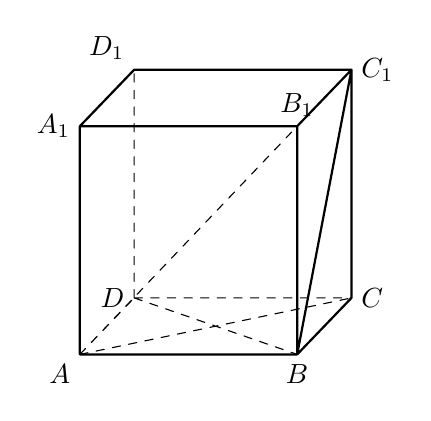
\begin{tikzpicture}[line cap=round,line join=round,scale=0.92]
  \coordinate (A)  at (0,0);
  \coordinate (B)  at (3,0);
  \coordinate (C)  at (3.75,0.78);
  \coordinate (D)  at (0.75,0.78);
  \coordinate (A1) at (0,3.15);
  \coordinate (B1) at (3,3.15);
  \coordinate (C1) at (3.75,3.93);
  \coordinate (D1) at (0.75,3.93);

  % 隐藏棱与题图中的辅助对角线
  \draw[dashed] (A)--(D) (D)--(C) (D)--(D1)
                (A)--(C) (D)--(B) (A)--(B1);
  % 棱柱可见棱及题设线段 BC_1
  \draw[thick] (A)--(B) (B)--(C) (A)--(A1) (B)--(B1) (C)--(C1)
               (A1)--(B1) (B1)--(C1) (C1)--(D1) (D1)--(A1)
               (B)--(C1);

  \node[below left] at (A) {$A$};
  \node[below] at (B) {$B$};
  \node[right] at (C) {$C$};
  \node[left] at (D) {$D$};
  \node[left] at (A1) {$A_1$};
  \node[above] at (B1) {$B_1$};
  \node[right] at (C1) {$C_1$};
  \node[above left] at (D1) {$D_1$};
\end{tikzpicture}
